\chapter{Podstawy teoretyczne}

Problem kategoryzacji obrazów wpisuje się w dziedzinę rozpoznawania obrazów. Zadanie to polega na rozpoznaniu przynależności różnych rodzajów obiektów do pewnych klas\cite{Tad91} i jest częścią większego zagadnienia, które określa się jako uczenie maszynowe.

\section{Uczenie maszynowe}

Uczenie maszynowe jest zagadnieniem interdyscyplinarnym z pogranicza informatyki, statystyki i sztucznej inteligencji, które zajmuje się tworzeniem systemów mogących doskonalić się za pomocą dostarczanych danych.

Systemy te ulegają nieustannej modyfikacji, zmieniają swoje wewnętrzne parametry po to by osiągnąć korzyści takie jak zwiększenie efektywności lub wydajności działania. Ważną cechą jest to, że jakkolwiek zmiany te zachodzą na podstawie czynników zewnętrznych to jednak dokonują się w~systemie autonomicznie. System, który się uczy zmienia sam siebie na lepsze.\cite{CICHOSZ00}

\section{Uczenie nadzorowane i nienadzorowane}

W uczeniu maszynowym możemy wyróżnić dwa zasadnicze podejścia: uczenie nadzorowane (\emph{ang. supervised machine learning}) i nienadzorowane (\emph{ang. unsupervised machine learning}). Różnica pomiędzy nimi polega na obecności w uczeniu nadzorowanym tzw. nauczyciela, który stanowi źródło informacji trenującej. Posługując się analogiczną terminologią, system który podlega nauce określa się jako ucznia. Na rys. \ref{fig:supervised-learning} przedstawiono schemat uczenia maszynowego z użyciem nauczyciela.

\begin{figure}[h]
	\centering
	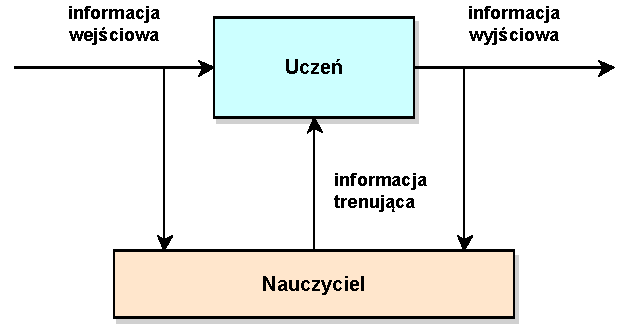
\includegraphics{graphics/01_podstawy_teoretyczne/supervised-learning.pdf}
	\caption{Uczenie maszynowe z nauczycielem \cite{CICHOSZ00}}
	\label{fig:supervised-learning}
\end{figure}

Uczeń otrzymuje od nauczyciela informację o tym jakiego komunikatu wyjściowego oczekuje w odpowiedzi na przykładowe informacje wejściowe. Mogą być one dostarczone np. w formie par składających się z wektorów danych oraz poprawnej odpowiedzi: $(x_{i}, y_{i})$. Na podstawie przykładów, system ma wyuczyć się przyporządkowywania danych do odpowiednich odpowiedzi. Innymi słowy, ma nauczyć się takiej funkcji $f$, dla której $f(x_{i})=y_{i}$, dla każdego $i$. Przykładami w uczeniu maszynowym mogą być różne obiekty, takie jak przedmioty, osoby, obserwacje.

Każdy przykład określany jest przez skończony oraz niepusty zbiór atrybutów $A=\lbrace a_{i}, a_{2}, \cdots, a_{n}\rbrace$. Atrybuty ze względu na rodzaj dziedziny możemy podzielić na: 
\begin{compactitem}
	\item nominalne, tj. takie, których dziedziny są zbiorami nieuporządkowanymi - dla dwóch wartości możliwe jest określenie jedynie czy są równe czy nierówne,
	\item porządkowe, dla których dziedziny są zbiorami uporządkowanymi, czyli możliwe jest określenie relacji porządku liniowego na zbiorze wartości,
	\item liczbowe, których dziedziny są zdefiniowane jako zbiór liczbowy.
\end{compactitem}

W zależności od rodzaju odpowiedzi możemy wyróżnić dwa typowe rodzaje problemów, które stara się rozwiązać uczenie nadzorowane. Jeśli system ma przyporządkować do wektora wejściowego pojedynczą kategorię pochodzącą ze skończonego i dyskretnego zbioru kategorii, wówczas określamy ten problem jako problem kategoryzacji. Natomiast w przypadku przyporządkowywania odpowiedzi składającej się z jednej lub więcej zmiennych ciągłych, mówimy o problemie regresji.\cite{BISHOP06} Proces działania maszyny realizującej uczenie nadzorowane możemy podzielić na dwa etapy: etap treningu lub też nauki oraz etap polegający na rozwiązywania przynależności nowych wektorów wejściowych, który często określa się jako testowanie lub walidację.

W uczeniu nienadzorowanym nie występuje rola nauczyciela, a co za tym idzie, do systemu nie trafiają informacje treningowe. Dostępne są jedynie wektory wejściowe i na podstawie ich obserwacji system ma nauczyć się odpowiednich odpowiedzi.\cite{CICHOSZ00} Podejście to nie polega zatem na przyporządkowaniu wektorów do ustalonych wcześniej kategorii, lecz na wyznaczeniu ukrytej struktury w danych, które są nieopisane.\cite{VALPOLA} Wykorzystywane jest m.in. do rozwiązywania problemu klasteryzacji (\emph{ang. clustering}), który polega na znajdowaniu grup podobnych obiektów wśród danych wejściowych. Ponadto uczenie nienadzorowane wykorzystywane jest to określania rozkładu danych w przestrzeni wejściowej, co nazywamy szacowaniem rozkładu (\emph{ang. density estimation}) lub do rzutowania danych z przestrzeni wielowymiarowej do trójwymiarowej w celu dokonania wizualizacji.\cite{BISHOP06}

Na rys. \ref{fig:unsupervised-learning} przedstawiono uproszczony schemat mechanizmu uczenia nienadzorowanego. Algorytm uczący dokonuje podziału zestawu danych na klastry, które następnie muszą zostać zinterpretowane przez człowieka. W zaprezentowanym przykładzie klastry zostały nazwane na podstawie analizy ich zawartości. W rzeczywistych problemach zadanie nadania etykiet wytworzonym klastrom może okazać się trudne i może wymagać dostrojenia parametrów algorytmu by identyfikacja klastrów była możliwa.

\begin{figure}[h]
	\centering
	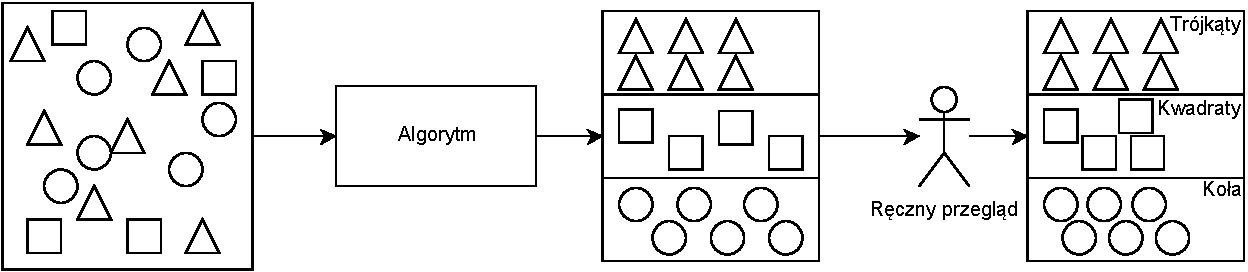
\includegraphics[scale=0.8]{graphics/01_podstawy_teoretyczne/unsupervised-learning.pdf}
	\caption{Uczenie maszynowe nienadzorowane \cite{CASEY}}
	\label{fig:unsupervised-learning}
\end{figure}

Dane wejściowe z etapu walidacji mogą się różnić od przykładowych danych służących do wytrenowania systemu. Umiejętność udzielania poprawnej odpowiedzi na komunikaty, które różnią się od przykładowych danych określamy jako generalizacja.\cite{BISHOP06}
%TODO napisac o tym w kontekscie pracy, co raczej sie nadaje a co raczej nie

Wśród dostępnych publikacji na temat kategoryzacji obrazów przeważają rozwiązania oparte na uczeniu nadzorowanym lub pól-nadzorowanym.\cite{MELE06}\cite{CHEN04}\cite{Vitaladevuni13}\cite{LUO11} Istnieje jednak kilka rozwiązań opartych na uczeniu nienadzorowanym, m.in. w  Dai D., Wu T., Zhu S-c., \emph{Discovering Scene Categories by Information Projection and Cluster Sampling}\cite{DAI10} gdzie zaprezentowano metodę kategoryzacji sceny opartą na uczeniu nienadzorowanym, lub Huang Y., Liu Q., Lv F., Gong Y., Dimitris N., \emph{Unsupervised Image Categorization by Hypergraph Partition}\cite{HUANG11}, gdzie klastrowanie obrazów sformowano jako problem podziału hipergrafu.

\section{Rozpoznawanie wzorców}

%TODO sprawdzic wzory

Celem rozpoznawania wzorców (\emph{ang. pattern recognition}) jest stworzenie symbolicznego opisu dla zawartości jedno lub wielowymiarowego sygnału cyfrowego takiego jak np. cyfrowy obraz graficzny, sygnał mowy, lub obraz z kamery, a następnie przyporządkowanie do niego klasy lub instancji klasy. Opis ten może być zrealizowany w różnej formie: funkcji, obiektów, ruchu, wyrazów lub struktur.

Wzorcem nazywamy zbiór cech, który tworzy ilościowy oraz jakościowy opis obiektu. Wzorce zapisujemy najczęściej jako wektory, ciągi lub drzewa. Wzór \ref{pattern_vector} przedstawia wektor cech, gdzie $x_{i}$ reprezentuje $i$-tą cechę, a $n$ oznacza ilość wszystkich cech powiązanych ze wzorcem.\cite{GONZALES01}
\begin{equation} 
\label{pattern_vector} 
\overrightarrow{x}=
\begin{bmatrix}x_1\\
x_2\\
\vdots\\
x_n  
\end{bmatrix}
\end{equation}

Zbiór wzorców charakteryzujący się podobnymi wektorami cech nazywamy klasą wzorców i oznaczamy jako $\omega_1, \omega_2, \cdots, \omega_{W}$, gdzie dolny indeks określa numer klasy, a $W$ określa ilość klas. Jako rozpoznanie wzorca $\omega$ określa się przyporządkowanie wzorcowi jego klasy: $\overrightarrow{x} \rightarrow \omega$. Przestrzeń wektorów cech $X$ zostaje przekształcona w przestrzeń klas wzorców $\Omega$.

W systemach analizy obrazów możemy oprócz rozpoznania zdefiniować również dwa inne pojęcia: identyfikację oraz weryfikację. Gdy nie dysponujemy opisami klas wzorców, a jedynie przechowujemy wzorce referencyjne, celem systemu jest porównanie aktualnego wzorca z bazą referencyjną. Jeśli na podstawie określonej odległości pomiędzy parami wzorców system jest w stanie dokonać wyboru dokładnie jednego wzorca referencyjnego, to określamy takie rozwiązanie jako identyfikację. Natomiast jeśli możemy wybrać przynajmniej jeden ze wzorców referencyjnych to określamy takie rozwiązanie jako weryfikację.

\section{Selekcja cech}

%TODO sprawdzic wzory

W przypadku dużych i skomplikowanych obiektów, takich jak obrazy, proces uczenia może okazać się bardzo skomplikowany i czasochłonny. Konieczne jest przeprowadzenie procesu selekcji cech obrazu (\emph{ang. feature selection}), który polega na znalezieniu podzbioru cech opisujących obiekt w najlepszy sposób i zapewniający najwyższą jakość modelu klasyfikacji. Celem selekcji cech jest redukcja wymiarów przestrzeni cech, zwiększenie szybkości działania algorytmu uczącego, zwiększenie dokładności klasyfikacji oraz osiągnięcie łatwiejszych do zrozumienia rezultatów uczenia.\cite{MOTODA98}

Wyselekcjonowane cechy powinny się charakteryzować następującymi właściwościami\cite{STRUMIL}:

\begin{compactitem}
	\item \emph{dyskryminacja} - cechy powinny przyjmować jak najbardziej odmienne wartości dla obiektów z różnych klas,
	\item \emph{niezawodność} - cechy powinny przyjmować podobne wartości dla wszystkich obiektów danej klasy,
	\item \emph{niezależność} - cechy powinny nie być ze sobą skorelowane,
	\item \emph{małoliczność} - im mniejsza liczba cech tym złożoność systemu jest mniejsza.
\end{compactitem}

Wzór \ref{correlation} przedstawia współczynnik korelacji cech $x$ i $y$. Jeśli współczynnik korelacji jest bliski $1$ lub $-1$ to cechy $x$ i $y$ są ze sobą silnie skorelowane i należy jedną z nich odrzucić.
\begin{equation} 
\label{correlation} 
\hat{\sigma}_{xy}= \frac{\frac{1}{P}\sum\limits_{i=1}^P(x_i-\mu_x)(y_i-\mu_y)}{ \hat{\sigma}_x\hat{\sigma}_y }
\end{equation}

Gdzie $P$ - liczba klasyfikowanych obiektów, $\mu$ - wartość średnia, $\sigma$ - odchylenie standardowe zbioru cech.

Miarę separacji można określić jako:

\begin{equation}
	\hat{D}_{xjk} = \frac{|\mu_xj - \mu_xk|}{\sqrt{\hat{\sigma}^2_xj \hat{\sigma}^2_xk}}
\end{equation}

Duża wartość tej miary świadczy o dobrej separacji pomiędzy klasami $j$ i $k$.

Badanie jakości klasyfikacji dla wszystkich możliwych kombinacji podzbioru cech dla dużej liczby $N$ wszystkich cech jest bardzo kosztowne, dlatego w praktyce zbiór cech często dobierany jest intuicyjnie.\cite{STRUMIL}

%TODO Opis mRMR, CFS, http://en.wikipedia.org/wiki/Feature_selection

Po poprawnej selekcji cech, możliwe powinno się stać stworzenie takiego modelu, w którym cechy nie dające informacji potrzebnej do klasyfikacji lub takie, które są nadmiarowe lub pogarszają jakość klasyfikacji zostały wyeliminowane. Dążymy przy tym do osiągnięcia najmniejszego możliwego wektora cech. Opierając się na mniejszym, mniej wymiarowym wektorze cech, potrzeba mniej przykładów do osiągnięcia dobrych wyników klasyfikacji.

\section{Ekstrakcja cech}

Obrazy w formie map bitowych reprezentowane są w pamięci komputera w postaci macierzy pikseli. Ilość danych jest dla klasyfikacji zbyt duża i zawiera wiele niepotrzebnych informacji. Dlatego przed przystąpieniem do procesu klasyfikacji należy wydobyć z obrazu pewne cechy. Proces przetwarzania obrazu w celu wydobycia cech określa się jako ekstrakcję cech (\emph{ang. feature extraction}).

Można wyróżnić wiele cech używanych w procesach przetwarzania obrazów, np. rozkład kolorów w formie histogramu, obecność niektórych elementów lub kształtów, liczba występowania podobnych obiektów, wielkość kształtów, morfologia, tekstura.

\section{Przegląd algorytmów do ekstrakcji cech}

Wśród popularnych metod ekstrakcji cech, stosowanych do rozwiązania problemu klasyfikacji i kategoryzacji obrazów należy wymienić: SIFT (\emph{ang. Scale-invariant Feature Transform})\cite{SIFT99}, SURF (\emph{ang. Speeded Up Robust Features}), GIST\cite{GIST09}, LBP (\emph{ang. Local Binary Patterns}), HOG (\emph{ang. Histograms of Oriented Gradients}). Poszczególne algorytmy zostały opisane poniżej.

\subsection{SIFT - Scale-invariant Feature Transform}

Algorytm SIFT służy do wykrywania oraz opisu lokalnych cech obrazu, został opublikowany przez Dawida Lowe w 1999 roku.\cite{SIFT99} Cechy ekstraktowane przez SIFT są niezależne od położenia, rotacji, skali, zmiany oświetlenia oraz są odporne na zakłócenia. Zastosowanie algorytmu SIFT do rozpoznawania obiektów pozwala na detekcję częściowo zasłoniętych obiektów. Jest to jeden z najpopularniejszych algorytmów do ekstrakcji punktów charakterystycznych.

Działanie algorytmu rozpoczyna się od wyszukiwania potencjalnych punktów poprzez przetworzenie obrazu filtrem Gaussa w różnych skalach. Wzór \ref{sift_scale_space} przedstawia postać obrazu po przetworzeniu:
\begin{equation} 
\label{sift_scale_space} 
L(x, y, \sigma) = G(x, y, \sigma) \ast I(x, y)
\end{equation} gdzie $G(x, y, \sigma)$ - Gaussian, $I(x, y)$ obraz wejściowy, $\ast$ - operator splotu.
\begin{equation} 
\label{sift_gaussian} 
G(x, y, \sigma) = \frac{1}{2\pi\sigma^2}e^{-(x^2+y^2)/2\sigma^2}
\end{equation} 

Różnicowy filtr Gaussa (DOG) dla dwóch skali rozdzielonych współczynnikiem $k$ można zapisać jako:
\begin{equation} 
\label{sift_dog} 
G(x, y, k\sigma) - G(x, y, \sigma) 
\end{equation} 

Stąd wynik spotu obrazu z filtrem DOG można zapisać jako:
\begin{equation} 
\label{sift_splot} 
	\begin{gathered}
		D(x, y, \sigma) = [G(x, y, k\sigma) - G(x, y, \sigma)] \ast I(x, y) \\
		D(x, y, \sigma) = L(x, y, k\sigma) - L(x, y, \sigma)
	\end{gathered}
\end{equation}

Na rys. \ref{fig:sift-gaussian-to-dog} przedstawiono efektywny sposób konstruowania $D(x, y, \sigma)$. Obraz wejściowy fitrowany jest filtrem Gaussa w różnych skalach rozdzielonych stałym współczynnikiem $k$, a następnie na obliczane są obrazy różnicowe DOG. Każda oktawa jest dzielona na liczbę całkowitą $s$, określającą liczbę interwałów, więc $k=2^{1/s}$. Należy zatem wyprodukować $s+3$ obrazy dla każdej oktawy, tak aby końcowe ekstremum pokrywało całą oktawę. Procedurę powtarza się próbkując obraz gaussowski poprzez usunięcie co drugiego wiersza i kolumny obrazu.\cite{LOWE04}

\begin{figure}[h]
	\centering
	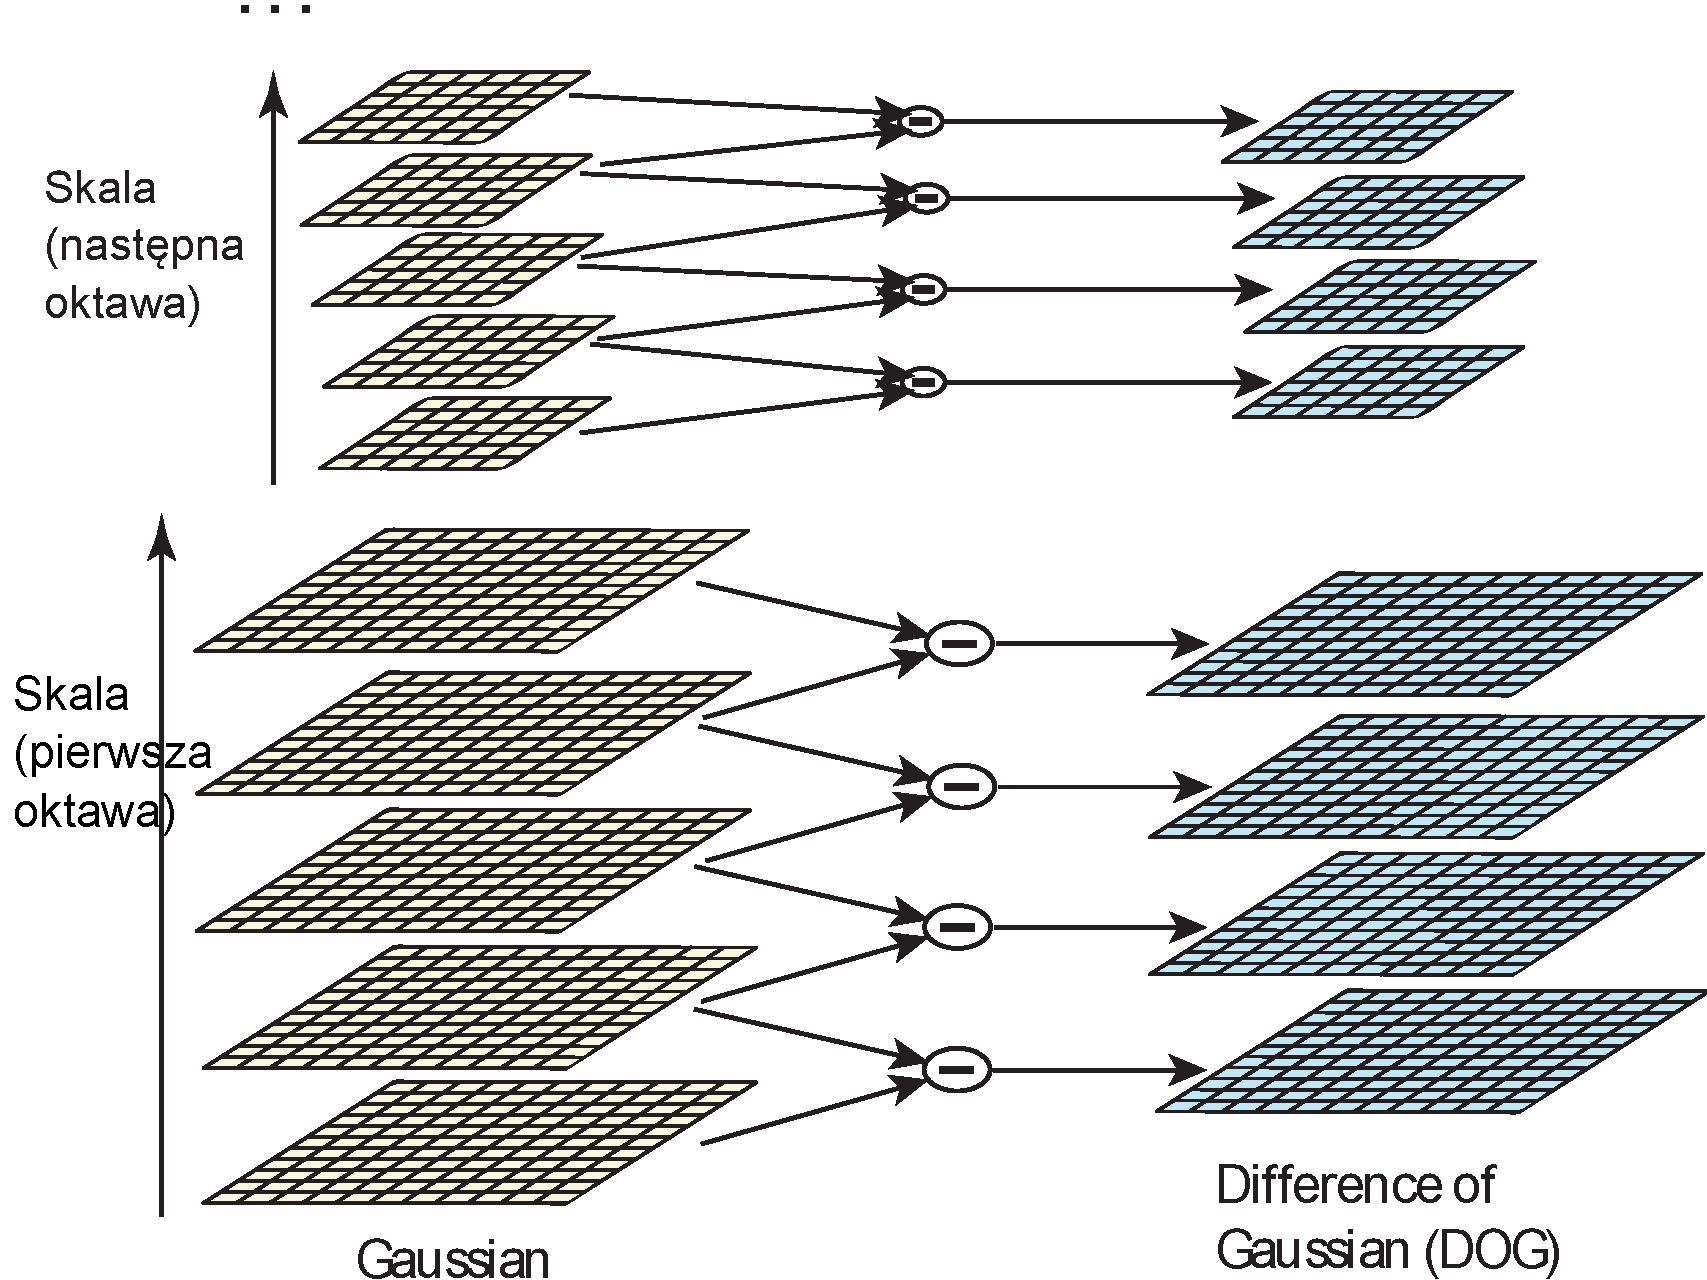
\includegraphics[scale=0.4]{graphics/01_podstawy_teoretyczne/sift-gaussian-to-dog.pdf}
	\caption{Proces tworzenia różnicy Gaussianów \cite{LOWE04}}
	\label{fig:sift-gaussian-to-dog}
\end{figure}

W celu wykrycia lokalnych ekstremów, punkty są porównywane z sąsiadami w otoczeniu 3x3x3, tj. po dziewięć sąsiadów w skalach poniżej i powyżej oraz z ośmioma sąsiadami w aktualnej skali. Punkt jest przyjmowany jako kandydat na punkt charakterystyczny tylko wówczas gdy ma wartość mniejszą lub większą od wszystkich 26 punktów sąsiednich.\cite{LOWE04} Rys. \ref{fig:sift-gaussian-min-max} przedstawia porównanie punktu, oznaczonego na schemacie za pomocą "X", z punktami sąsiednimi.

\begin{figure}[h]
	\centering
	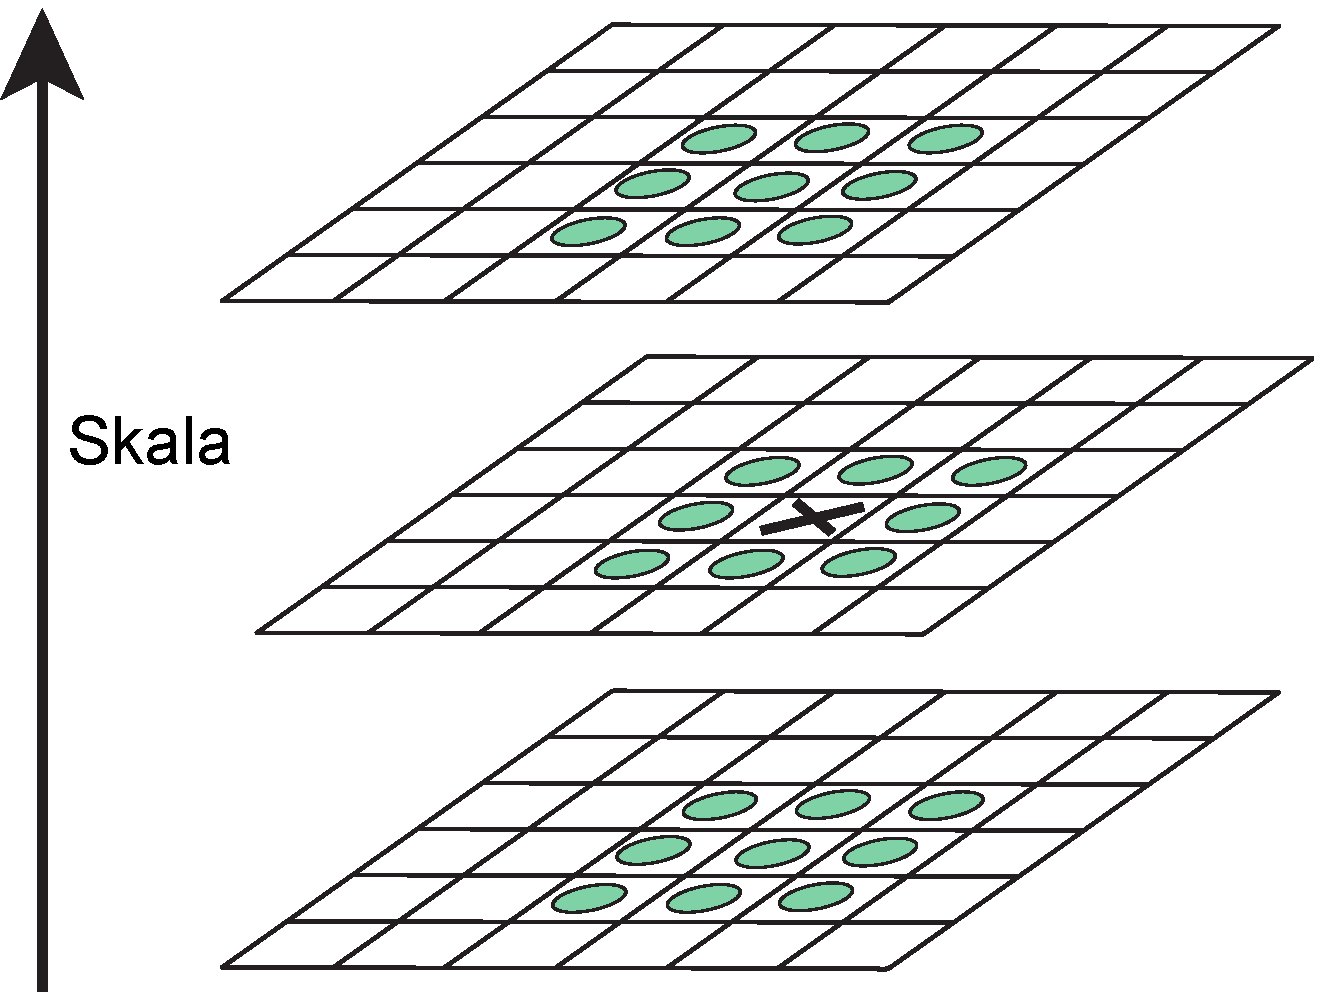
\includegraphics[scale=0.4]{graphics/01_podstawy_teoretyczne/sift-gaussian-min-max.pdf}
	\caption{Porównanie punktu z sąsiadami \cite{LOWE04}}
	\label{fig:sift-gaussian-min-max}
\end{figure}

Po znalezieniu kandydatów następuje lokalizacja punktów charakterystycznych. Proces ten odbywa się poprzez interpolację ekstremów dla kandydatów wyznaczonych w poprzednim punkcie za pomocą funkcji kwadratowej 3D:
\begin{equation} 
\label{sift_3d} 
D(x) = D + \frac{\partial D^T}{\partial x} x + \frac{1}{2}x^T \frac{\partial^2 D}{\partial x^2} x
\end{equation}

Dokładne położenie ekstremum wyznacza się na podstawie pochodnej funkcji $D(x)$:
\begin{equation} 
\label{sift_pochodna_D} 
\hat{x} = -\frac{\partial^2 D^-1}{\partial x^2}\frac{\partial D}{\partial x}
\end{equation}

Wartość funkcji w punkcie ekstremum służy do odrzucania niestabilnych punktów ze względu na mały kontrast. Wzór można uzyskać poprzez podstawienie wzoru \ref{sift_pochodna_D} do \ref{sift_3d}:
\begin{equation} 
\label{sift_Dx} 
D(\hat{x}) = D + \frac{1}{2} \frac{\partial D^T}{\partial x} \hat{x}
\end{equation}

Funkcja DOG będzie mieć dużą odpowiedź wzdłuż krawędzi. Za Harris i Stephens (1988), punkty ekstremum będące odpowiedzią wzdłuż krawędzi na obrazie są odrzucane na podstawie warunku \ref{sift_warunek}:
\begin{equation} 
\label{sift_warunek} 
\frac{\Tr(\boldsymbol{H})^2}{\Det(\boldsymbol{H})} < \frac{(r+1)^2}{r}
\end{equation} gdzie Hessian ma postać macierzy:
\begin{equation} 
\label{sift_hessian} 
\boldsymbol{H} = 
	\begin{bmatrix}
		D_{xx} & D_{xy} \\
		D_{xy} & D_{yy}
	\end{bmatrix}
\end{equation} oraz r jest stosunkiem największej wartości własnej macierzy do najmniejszej.

Orientacja punktów wyznaczana jest na podstawie jednego z obrazów gaussowskich, którego skala odpowiada skali danego punktu charakterystycznego. Dla każdej próbki obrazu $L(x, y)$ obliczne są moduł gradientu $m(x, y)$ oraz orientacja $\theta(x, y)$:
\begin{equation} 
\label{sift_gradient_magnitude} 
m(x, y) = \sqrt{(L(x + 1, y) - L(x - 1, y))^2 + (L(x, y + 1) - L(x, y - 1))^2}
\end{equation}

\begin{equation} 
\label{sift_orientation} 
\theta(x, y) = \tan^{-1}((L(x, y + 1) - L(x, y - 1))/L(x + 1, y) - L(x - 1, y)))
\end{equation}

Na podstawie orientacji punktów, w otoczeniu punktu charakterystycznego budowany jest histogram orientacji. Maksimum w histogramie i lokalne maksima o wartościach powyżej 80\% największego określają orientację punktu charakterystycznego.

Przyjmuje się, że histogram posiada 36 pól, a dokładne położenie maksimum interpoluje się za pomocą paraboli korzystając z wartości sąsiednich histogramu.

Dzięki temu, że wszystkie cechy punktów charakterystyczne są mierzone w odniesieniu do tak wyznaczonej orientacji,	opis jest niezależny od rotacji.

SIFT do opisu cech wykorzystuje moduł gradientu oraz orientację z otoczenia 16x16 dla danego punktu charakterystycznego. Obszar ten jest dzielony na podregiony 4x4, w których również wyznacza się wypadkowe histogramy orientacji. W każdym obszarze dla 8 orientacji wyznacza się wypadkowy moduł gradientu na podstawie modułów poszczególnych punktów. Na rys. \ref{fig:sift-descriptor} został przedstawiony przykład wyznaczenia wypadkowego gradientu dla otoczenia 8x8 i podregionów 2x2.

\begin{figure}[h]
	\centering
	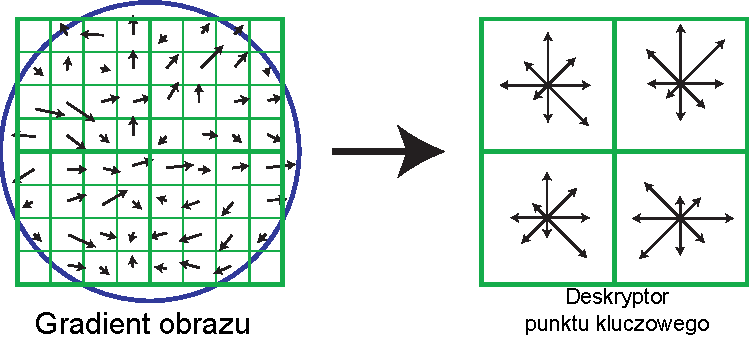
\includegraphics[scale=1]{graphics/01_podstawy_teoretyczne/sift-descriptor.pdf}
	\caption{Wyznaczenie deskryptora 2x2 z otoczenia 8x8 \cite{LOWE04}}
	\label{fig:sift-descriptor}
\end{figure}

W celu rozpoznania obiektów za pomocą algorytmu SIFT należy najpierw wyznaczyć punkty charakterystyczne i odpowiadające im wektory cech lokalnych, a następnie dopasować punkty charakterystyczne z obrazu wejściowego do punktów w bazie wzorców. Do identyfikacji grup dopasowanych punktów, które określają ten sam obiekt wykorzystuje się transformatę Hougha. Weryfikacji cech dokonuje się z wykorzystaniem metody najmniejszych kwadratów. W trakcie obliczeń wyznaczane są parametry związane z transformacją pomiędzy układem związanym z wzorcem a układem związanym z obiektem na badanym obrazie.

\subsection{SURF - Speeded Up Robust Features}

SURF jest kolejnym algorytmem do wykrywania lokalnych cech obrazu. Został zaproponowany w 2006 roku przez Herberta Bay'a i jest częściowo wzorowany na algorytmie SIFT.\cite{BAY08} Algorytm jest odporny zarówno na zmiany skali jak i zmiany rotacji. Wykorzystywany jest do rozpoznawania obiektów jak i rekonstrukcji scen 3D. Typowa implementacja jest nawet kilka razy szybsza od algorytmu SIFT.\cite{SCHWEIGER09}

W celu optymalizacji działania filtrów splotowych zastosowano obrazy całkowe (\emph{ang. integral images}). Pozycja w obrazie całkowym $I_{\Sigma}(\boldsymbol{x})$ w punkcie $\boldsymbol{x}=(x, y)^T$ reprezentuje sumę wszystkich pikseli wejściowego obrazu $I$ wewnątrz prostokąta pomiędzy początkiem układu współrzędnych a $x$.
\begin{equation} 
\label{surf_integral_image} 
I_{\Sigma}(\boldsymbol{x}) = \sum\limits_{i=0}^{i \leq x} \sum\limits_{j=0}^{j \leq y} I(i,j)
\end{equation}

Zastosowanie obrazu całkowego (\emph{ang. integral image}) pozwala ograniczyć ilość operacji dla sumowania intensywności oraz uniezależnić czas obliczeń od wielkości filtra.\cite{BAY08}

Ze względów wydajnościowych, wyszukiwanie punktów charakterystycznych oparte zostało na Hessianie. Dla punktu $\boldsymbol{x}=(x, y)$ na obrazie $I$, Hessian $H(\boldsymbol{x}, \sigma)$ w punkcie $\boldsymbol{x}$ i w skali $\sigma$ został zdefiniowany we wzorze \ref{surf_hessian}.
\begin{equation} 
\label{surf_hessian} 
H(\boldsymbol{x}, \sigma) = 
	\begin{bmatrix}
		L_{xx}(\boldsymbol{x}, \sigma) & L_{xy}(\boldsymbol{x}, \sigma) \\
		L_{xy}(\boldsymbol{x}, \sigma) & L_{yy}(\boldsymbol{x}, \sigma)
	\end{bmatrix}
\end{equation} gdzie $L_{xx}(\boldsymbol{x}, \sigma)$ - splot drugiej pochodnej Gaussiana $\frac{\partial^2}{\partial x^2} g(\sigma)$ z obrazem $I$ w punkcie $\boldsymbol{x}$.

O ile zastosowanie Gaussianów jest optymalne\cite{LINDENBERG90}, to jednak ma obniżoną powtarzalność przy rotacji dla nieparzystych wielokrotności $\frac{\pi}{2}$. Korzystając z tych obserwacji, w algorytmie SURF zaproponowano przybliżenie oparte na filtrze pudełkowym. Na rys. \ref{fig:surf-box-filters} zostało przedstawione porównanie pochodnej drugiego rzędu w $L_{yy}$ (a), $L_{xy}$ (b), przybliżenie $D_{yy}$ (c) oraz $D_{xy}$ (d).

\begin{figure}[h]
	\centering
	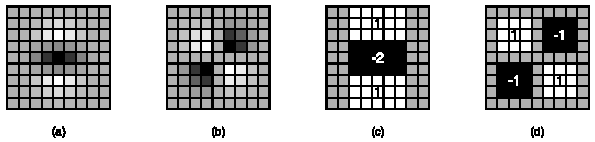
\includegraphics[scale=1.7]{graphics/01_podstawy_teoretyczne/surf-box-filters.pdf}
	\caption{Porównanie filtra Gaussa z filtrem pudełkowym 9x9 ($\sigma = 1.2$) \cite{BAY08}}
	\label{fig:surf-box-filters}
\end{figure}

Wyznacznik przybliżonej wartości Hessiana $H$ można zapisać jako:
\begin{equation} 
\label{surf_hessian_det}
\det(H_{approx}) = D_{xx} D_{yy} - (w D_{xy})^2
\end{equation}

Waga odpowiedzi filtra $w$ służy do zrównoważenia wyrażenia, dla zachowania energii pomiędzy jądrem Gaussiana a jądrem przybliżonego Gaussiana.
\begin{equation} 
\label{surf_hessian_approx_w}
w = \frac{|L_{xy}(1.2)|_F |D_{yy}(9)|_F}{|L_{yy}(1.2)|_F |D_{xy}(9)|_F} = 0.912... \simeq 0.9
\end{equation} gdzie $|A|_F$ - norma Froberiusa (wzór \ref{surf_froberius}).
\begin{equation} 
\label{surf_froberius}
|A|_F = \sqrt{\sum\limits_{i=1}^m \sum\limits_{j=1}^n |a_{ij}|^2}
\end{equation}

Ze względu na teoretyczną dokładność, wagi $w$ powinny zmieniać się wraz ze skalą, jednakże w praktyce nie ma to dużego wpływu na precyzję wyników, w związku z tym przyjmuje się stałe $w$. Przybliżone wyznaczniki Hessianów reprezentują odpowiedź obszarów spójnych ({ang. blob}) w punkcie $x$.

\subsection{GIST}

\subsection{LBP - Local Binary Patterns}

\subsection{HOG - Histograms of Oriented Gradients}


\section{Klasyfikacja}
%TODO wymienic rozne rodzaje klasyfikatorow
%https://www.youtube.com/watch?v=qdDHp29QVdw
...


\subsection{Klasyfikator według funkcji potencjału}
...
	
\subsection{Klasyfikator statystyczny Bayesa}
...
	
\subsection{Klasyfikator według minimalnej odległości}
...
	
\subsection{Klasyfikator k Najbliższych Sąsiadów}
...

\subsection{Maszyna wektorów wspierających (SVM)}
...
	
\section{Ocena klasyfikatorów}
...
